% Options for packages loaded elsewhere
\PassOptionsToPackage{unicode}{hyperref}
\PassOptionsToPackage{hyphens}{url}
%
\documentclass[
]{article}
\usepackage{amsmath,amssymb}
\usepackage{iftex}
\ifPDFTeX
  \usepackage[T1]{fontenc}
  \usepackage[utf8]{inputenc}
  \usepackage{textcomp} % provide euro and other symbols
\else % if luatex or xetex
  \usepackage{unicode-math} % this also loads fontspec
  \defaultfontfeatures{Scale=MatchLowercase}
  \defaultfontfeatures[\rmfamily]{Ligatures=TeX,Scale=1}
\fi
\usepackage{lmodern}
\ifPDFTeX\else
  % xetex/luatex font selection
\fi
% Use upquote if available, for straight quotes in verbatim environments
\IfFileExists{upquote.sty}{\usepackage{upquote}}{}
\IfFileExists{microtype.sty}{% use microtype if available
  \usepackage[]{microtype}
  \UseMicrotypeSet[protrusion]{basicmath} % disable protrusion for tt fonts
}{}
\makeatletter
\@ifundefined{KOMAClassName}{% if non-KOMA class
  \IfFileExists{parskip.sty}{%
    \usepackage{parskip}
  }{% else
    \setlength{\parindent}{0pt}
    \setlength{\parskip}{6pt plus 2pt minus 1pt}}
}{% if KOMA class
  \KOMAoptions{parskip=half}}
\makeatother
\usepackage{xcolor}
\usepackage[margin=1in]{geometry}
\usepackage{graphicx}
\makeatletter
\newsavebox\pandoc@box
\newcommand*\pandocbounded[1]{% scales image to fit in text height/width
  \sbox\pandoc@box{#1}%
  \Gscale@div\@tempa{\textheight}{\dimexpr\ht\pandoc@box+\dp\pandoc@box\relax}%
  \Gscale@div\@tempb{\linewidth}{\wd\pandoc@box}%
  \ifdim\@tempb\p@<\@tempa\p@\let\@tempa\@tempb\fi% select the smaller of both
  \ifdim\@tempa\p@<\p@\scalebox{\@tempa}{\usebox\pandoc@box}%
  \else\usebox{\pandoc@box}%
  \fi%
}
% Set default figure placement to htbp
\def\fps@figure{htbp}
\makeatother
\setlength{\emergencystretch}{3em} % prevent overfull lines
\providecommand{\tightlist}{%
  \setlength{\itemsep}{0pt}\setlength{\parskip}{0pt}}
\setcounter{secnumdepth}{5}
\usepackage{bookmark}
\IfFileExists{xurl.sty}{\usepackage{xurl}}{} % add URL line breaks if available
\urlstyle{same}
\hypersetup{
  pdftitle={Visualizing the Uninsured: A Data-Driven Perspective on U.S. Health Coverage},
  hidelinks,
  pdfcreator={LaTeX via pandoc}}

\title{Visualizing the Uninsured: A Data-Driven Perspective on U.S.
Health Coverage}
\author{Eduardo Sáenz-Messía Laborda, 2861597 Catherina Mikhail,
2847118\\
Charlotte Craenen, 2865572\\
Hugo van As, 2848225 Indy Pleijter\\
Julian Zeguers\\
Wies Polderman\\
Tutorial group 5, group 4 -- J.F. Fitzgerald}
\date{2025-06-24}

\begin{document}
\maketitle

{
\setcounter{tocdepth}{2}
\tableofcontents
}
\textbf{Part 1 -- Identify a Social Problem}

\subsection{1.1 Describe the Social
Problem}\label{describe-the-social-problem}

The large number of uninsured people in the United States represents a
significant social issue with serious consequences for individuals and
the healthcare system. As of 2022, over 27 million
Americans---approximately one in twelve people---lacked health insurance
coverage (KFF, 2023). This lack of coverage creates substantial barriers
to healthcare access and has wide-ranging effects on both personal and
public health.

For individuals without insurance, the consequences are often severe.
Uninsured people are much more likely to delay or avoid necessary
medical care due to cost concerns, which leads to worse health outcomes,
preventable emergency room visits, and higher rates of preventable
deaths. The financial impact is equally serious, as uninsured
individuals must pay full price for medical services, often resulting in
medical debt, damaged credit, and long-term financial hardship (Davis,
2007).

The problem extends beyond individual impacts to affect the entire
healthcare system. When uninsured patients cannot pay for their care,
hospitals and clinics must absorb these costs as uncompensated care.
This financial burden strains healthcare providers and ultimately
increases costs for everyone else through higher insurance premiums and
taxes. As Davis (2007) explains, the uninsured population includes ``our
neighbors, co-workers, and family members,'' making this a
community-wide issue that affects society as a whole.

\subsection{1.2 Provide Background on the
Problem}\label{provide-background-on-the-problem}

The Affordable Care Act (ACA), enacted in 2010, significantly expanded
health insurance coverage through Medicaid expansion and subsidized
insurance marketplaces. However, millions of Americans remain uninsured
despite these reforms. According to the Kaiser Family Foundation, most
uninsured individuals today are low-income workers, disproportionately
people of color, and residents of states that chose not to expand
Medicaid under the ACA (KFF, 2023).

A major factor contributing to this problem is the employment-based
nature of the U.S. health insurance system. Many uninsured individuals
work in jobs that do not offer health benefits, including part-time,
temporary, or service sector positions. These workers often earn too
much to qualify for traditional Medicaid but too little to afford
private insurance, creating what Davis (2007) describes as falling
``through the cracks'' of the current system.

Geographic disparities also play a significant role. States that
expanded Medicaid under the ACA have substantially lower uninsured rates
than non-expansion states, creating uneven access to coverage across the
country. This policy variation has resulted in particularly high
uninsured rates in many Southern and some Western states.

The persistence of uninsurance reflects broader structural challenges in
American healthcare, including affordability, accessibility, and policy
gaps that leave vulnerable populations without coverage options.

\section{Part 2 -- Describe and Acquire
Data}\label{part-2-describe-and-acquire-data}

\subsection{2.1 Describe the Data sets}\label{describe-the-data-sets}

This analysis utilizes two primary datasets to examine patterns in
health insurance coverage and their relationship to economic conditions
across U.S. states.

\textbf{U.S. Census Bureau Data} The main data set comes from the U.S.
Census Bureau's American Community Survey (ACS) 1-Year Estimates,
specifically the table ``Selected Characteristics of the Uninsured in
the United States.'' This data set covers the period from 2010 to 2023,
excluding 2020 due to the absence of 1-year estimates for that year.

Eight smaller states and territories were excluded from the
analysis---Delaware, District of Columbia, Hawaii, Puerto Rico, North
Dakota, Rhode Island, Vermont, and Wyoming---because they are not
consistently included in the 1-year estimates. The 1-year estimates were
chosen over 5-year estimates because they provide more timely data that
can capture short-term changes from economic shifts or policy reforms.

The ACS data set provides state-level information on the civilian
non-institutionalized population, including total population counts,
number of uninsured individuals, and various demographic and
socioeconomic characteristics. For this analysis, we focused on total
population figures and household income data (adjusted for inflation) to
calculate uninsured rates and understand the economic context.

\textbf{Bureau of Economic Analysis Data} Economic data comes from the
Bureau of Economic Analysis (BEA) table SAGDP1 -- State Annual Gross
Domestic Product Summary. This data set provides real GDP figures in
millions of chained 2017 dollars for each state from 1997 through 2024.
Using inflation-adjusted GDP enables consistent comparisons over time
and across different states.

\textbf{Data Integration} These two datasets together provide a
comprehensive view of how health insurance coverage has changed across
the United States over time and how coverage patterns may relate to
state-level economic conditions. The combination allows for analysis of
both temporal trends and cross-state variations in uninsured rates.

\subsection{2.2 Import and Prepare the Data
set}\label{import-and-prepare-the-data-set}

\textbf{First data set:} \textbf{``Selected Characteristics of The
Uninsured in the U.S.''}

\begin{itemize}
\tightlist
\item
  Here we imported the first data set from the U.S. Census Bureau and
  named them ``dataset\_uninsured\_population\_\emph{year''} from
  2010-2023, excl 2020.
\end{itemize}

\textbf{Second Data set: ``SAGDP1 State Annual Gross Domestic Product
Summary'', Statistic: ``Real GDP (millions of chained 2017 dollars)''}

\begin{itemize}
\tightlist
\item
  Here we imported the second data set from the Bureau of Economic
  Analysis of the annual GDP of the states from 2009-2023 and named it
  ``table\_GDP''
\end{itemize}

\subsection{Data cleaning: Data sets of Uninsured Population and The
Creation of The New Variable: The Uninsured
Share}\label{data-cleaning-data-sets-of-uninsured-population-and-the-creation-of-the-new-variable-the-uninsured-share}

To prepare the data for analysis, we began by removing all margins of
error from the original Census data sets. While margins of error are
important for assessing statistical precision, they were not necessary
for our purposes, which focused on comparing overall trends in health
insurance coverage across states and years. Removing them helped
simplify the data set and reduce complexity without compromising our
analytic goals.

A more structural challenge involved the inclusion of smaller states and
territories. Since 2016, the Census Bureau's 1-year estimates no longer
cover certain low-population areas, meaning they are missing from some
years in our timespan. To ensure consistency across time, we decided to
exclude eight such places entirely from our analysis. These were
Delaware, the District of Columbia, Hawaii, Puerto Rico, North Dakota,
Rhode Island, Vermont, and Wyoming. By removing them, we ensured that
our data set included only states that were present in every applicable
year from 2010 to 2023 (with the exception of 2020, when no data was
published due to the COVID-19 pandemic).

After resolving issues of consistency and coverage, we turned our
attention to the structure of the data itself. Each annual data set
included a wide range of metadata---demographic and socioeconomic
characteristics that, while valuable for other types of research, were
not essential to our primary analysis of insurance coverage trends. We
removed variables related to age, sex, race and Hispanic or Latino
origin, nativity and U.S. citizenship status, disability status,
residence one year ago, educational attainment, employment status, work
experience, civilian non-institutionalized workers aged 16 and over,
earnings in the past 12 months, and the ratio of income to the poverty
level in the past 12 months. From all this, we retained only the total
civilian non-institutionalized population and household income (adjusted
for inflation), which were directly relevant to our questions about
insurance and economic context.

To ensure the data was ready for calculations, we then converted all
numeric values that had been stored as character strings---often due to
formatting like commas---into actual numeric variables. This was a
necessary step for performing any reliable mathematical operations.

One of the most important transformations in our cleaning process was
the creation of a new variable: uninsured share. The original data
provided the total population and the total number of uninsured
individuals for each state and year. To make this more interpretable and
comparable, we calculated the uninsured share by dividing the number of
uninsured people by the total population and multiplying the result by
100. This gave us a percentage that reflects the proportion of each
state's population without health insurance. Expressing the data this
way allows for easier comparisons across time and across states,
regardless of differences in population size. It helps illuminate
broader patterns in insurance coverage that would be difficult to spot
using absolute numbers alone.

After all these cleaning and transformation steps, we combined the
individual yearly data sets into a single, comprehensive data set
covering the period from 2010 to 2023 (excluding 2020). This final
merged file allowed us to analyze long-term trends and relationships in
a consistent and structured way.

\subsection{Data cleaning: Annual GDP Table and The Creation of The New
Variable: Annual Real GDP Growth per year and
state}\label{data-cleaning-annual-gdp-table-and-the-creation-of-the-new-variable-annual-real-gdp-growth-per-year-and-state}

For the economic data from the Bureau of Economic Analysis, we worked
with the \emph{SAGDP1 -- State Annual Gross Domestic Product Summary}
table, which reports real GDP per state in millions of chained 2017
dollars. Before analysis, we cleaned this data set to align it with the
structure and timeframe of our health insurance data. First, we removed
all columns corresponding to years outside our scope---specifically,
1997 through 2008, as well as 2020 and 2024. We also filtered out states
and regions that were not included in our main data set or that
represented aggregate regions rather than individual states.
Specifically, we excluded Delaware, District of Columbia, Hawaii, North
Dakota, Puerto Rico, Vermont, Wyoming, and Rhode Island, as well as the
regional aggregates: New England, Mideast, Great Lakes, Plains,
Southeast, Southwest, Rocky Mountain, and Far West. Also here, the
values were stored as ``double'', so we coerced the values to numeric,
so that we are able to compute our new variable. After these
adjustments, we renamed the cleaned data set \texttt{table\_GDP} for use
in our analysis.

From this cleaned table, we created a new variable: annual real GDP
growth, calculated for each state and year by measuring the
year-over-year percentage change in real GDP. This variable allowed us
to capture how quickly or slowly each state's economy was growing over
time. Including GDP growth in our analysis adds important context: it
helps us explore whether changes in economic performance are linked to
shifts in health insurance coverage. For example, we can examine whether
periods of economic expansion correspond with improvements in coverage
rates. By combining this with our uninsurance data, we gain a more
nuanced understanding of how economic conditions may influence access to
healthcare.

\section{Part 3 -- Visualize and Analyze the
Data}\label{part-3-visualize-and-analyze-the-data}

\subsection{3.1 Create Initial
Visualizations}\label{create-initial-visualizations}

\textbf{Spatial Variation Visualization, U.S. Share of The Uninsured
Population in 2023}

\begin{itemize}
\tightlist
\item
  describe here that we mapped here the spatial variation of the
  uninsured population of the states of which we have the ACS one year
  estimates of and that we first created a subset of 2023 of the big
  dataset all\_states\_100 and that we plotted Alaska separately
  otherwise the whole map would be too small to visualize.
\end{itemize}

\pandocbounded{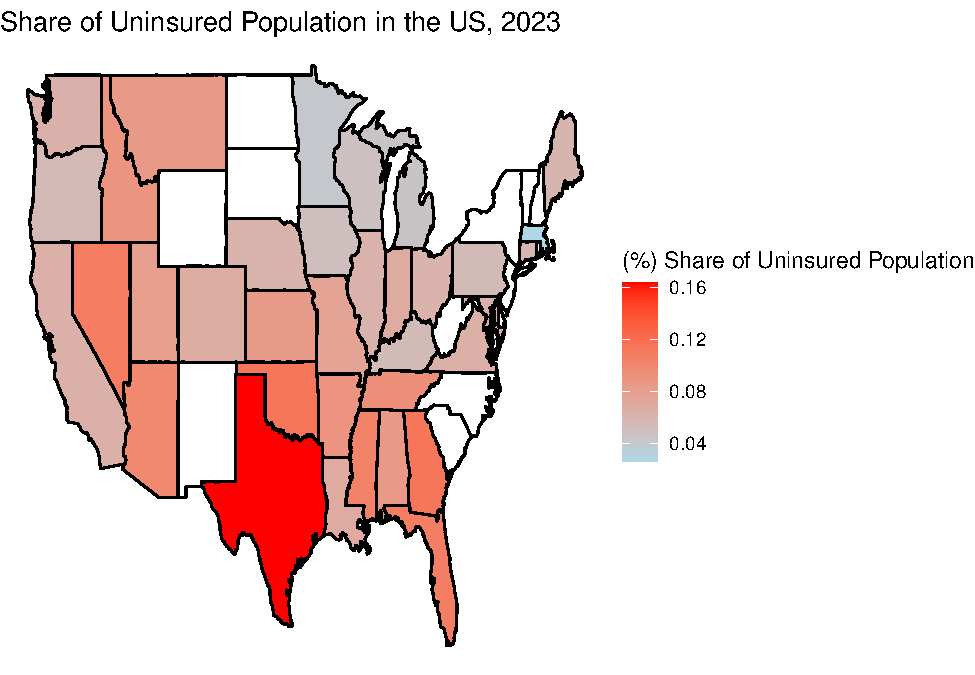
\includegraphics[keepaspectratio]{template_files/figure-latex/visualize spatial-1.pdf}}
\pandocbounded{
\includegraphics[keepaspectratio]{template_files/figure-latex/visualize spatial-2.pdf}}

\textbf{Temporal Variation Visualization, Texas's Share of Uninsured
Population and Texas's GDP growth rate over time}

\begin{itemize}
\tightlist
\item
  describe that Texas stood out in our spatial variation analysis and
  that we wanted to dig deeper into Texas's share of uninsured
  population over time from 2010 until 2023, except for 2020 and that we
  wanted to see if economic growth played a role in this.
\end{itemize}

\pandocbounded{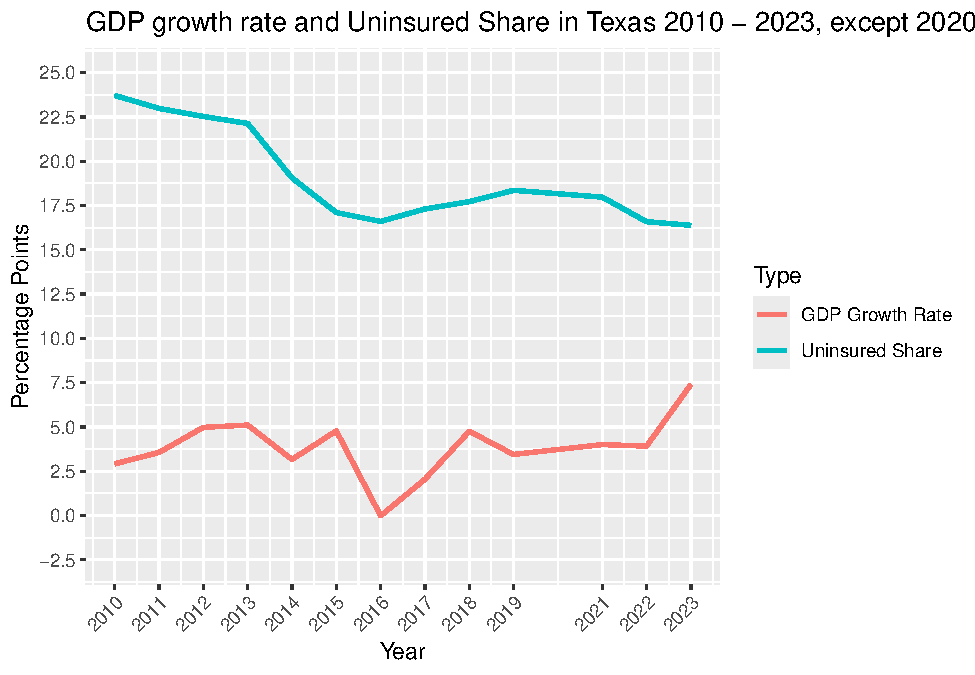
\includegraphics[keepaspectratio]{template_files/figure-latex/visualization temporal-1.pdf}}

\textbf{Sub-Group Variation Visualization, The Uninsured Rates of the
Middle-Income Group in 2017 in the U.S.}

\begin{itemize}
\tightlist
\item
  describe that already the KFF (2024) found that the uninsured people
  in the US are more likely to be low income and that we were wondering
  what the state of the middle-income group is as they earn too much for
  Medicaid but not enough for private insurance. 2017 is the year after
  Trump became president in 2016.
\end{itemize}

\begin{verbatim}
## [1] "First quartile (Q1): 26.625"
\end{verbatim}

\begin{verbatim}
## [1] "Second quartile (Q2): 29.35"
\end{verbatim}

\begin{verbatim}
## [1] "Third quartile (Q3): 31.25"
\end{verbatim}

\pandocbounded{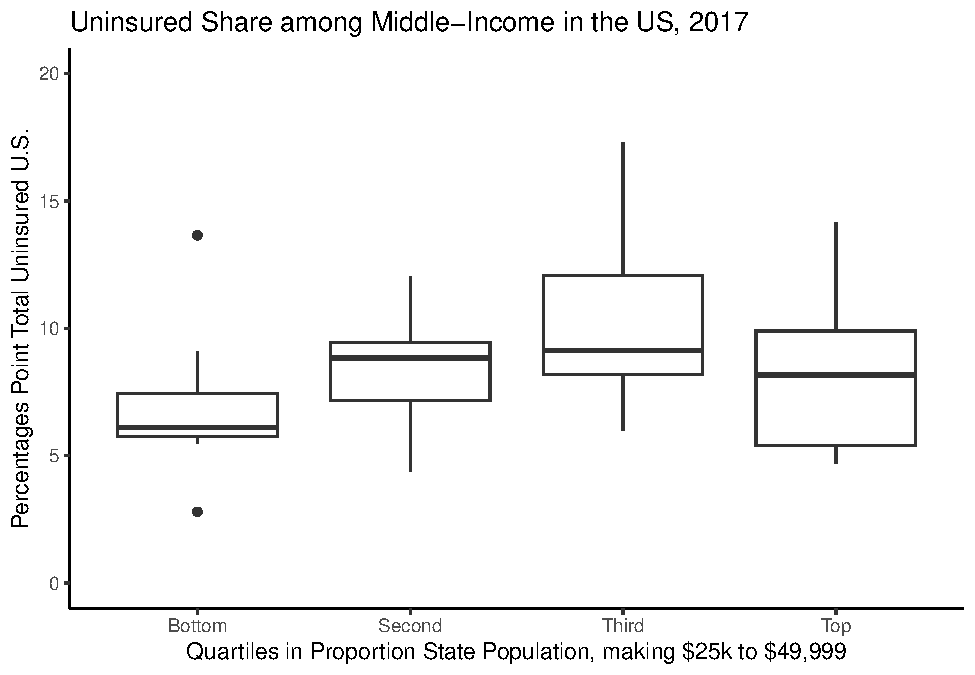
\includegraphics[keepaspectratio]{template_files/figure-latex/visualization subgroup-1.pdf}}

\textbf{Event Analysis Visualization, The Impact of The Implementation
of Work Requirements for Medicaid in Arkansas, 2018}

\begin{itemize}
\tightlist
\item
  describe here what happened in Arkansas in 2018 and why the wanted to
  implement the work requirements and what these requirements were. and
  that Arkansas is the treatment group and the other 43 states are the
  control group and the ware analysing if the implementation had
  significant impact on the uninsured rates compared to the change in
  the control group which is the weighted average of the uninsured
  rates.
\end{itemize}

\pandocbounded{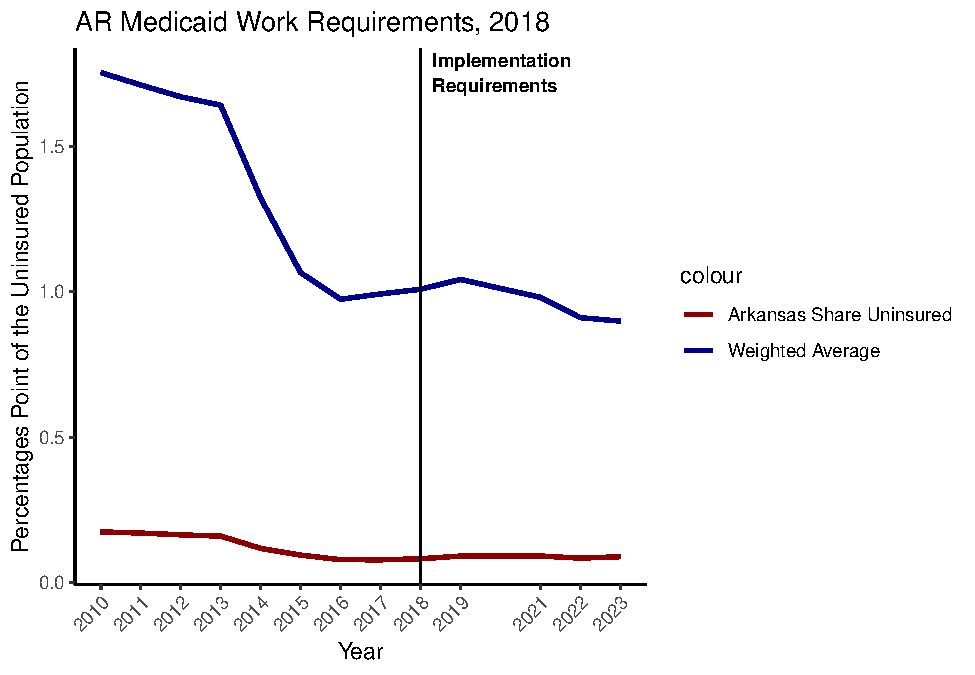
\includegraphics[keepaspectratio]{template_files/figure-latex/visualization event-1.pdf}}

\subsection{3.2 Identify Trends and
Patterns}\label{identify-trends-and-patterns}

\textbf{Spatial Variation Visualization, U.S. Share of The Uninsured
Population in 2023}

The spatial distribution of uninsured rates across the U.S. in 2023
reveals a stark regional divide. States in the South, especially Texas
and Florida, report the highest uninsured shares. In contrast,
Northeastern and Upper Midwestern states show much lower rates, likely
due to more expansive Medicaid programs, higher employer-based coverage,
and more generous state-level health initiatives (Bailey et al., 2017).

More nuanced is the case of Western states like Nevada and Arizona,
which also exhibit elevated uninsured rates despite having relatively
progressive policy environments. This may reflect labor market
characteristics---such as a higher prevalence of gig work, part-time
jobs, and self-employment---which are often associated with lower access
to employer-sponsored insurance (Collins et al., 2020). Furthermore,
undocumented immigrant populations, more common in some Western and
Southern states, are often excluded from public coverage (KFF, 2023),
further contributing to uninsured rates.

The findings support existing literature showing that health coverage in
the U.S. is not solely driven by state policy, but is deeply intertwined
with employment structures, income levels, and demographic profiles
(Davis, 2007; Sommers et al., 2012). Thus, even among states with
similar political leanings, uninsured rates can diverge significantly
based on labor and population dynamics.

\textbf{Temporal Variation Visualization, Texas's Share of Uninsured
Population and Texas's GDP growth rate over time}

The line graph illustrates the relationship between GDP growth rate and
the uninsured share in Texas from 2010 to 2023 (excluding 2020).

We observe a clear downward trend in the uninsured share, falling from
about 23\% to 17\% over this period. However, despite economic
fluctuations---particularly a dip in GDP growth around 2016 and a spike
in 2023---the uninsured rate remained relatively high and stable,
especially after 2016.

This pattern suggests that economic growth alone doesn't guarantee
increased health insurance coverage. Even in years with strong GDP
growth, Texas continued to have one of the highest uninsured rates in
the country. A likely explanation is Texas's decision not to expand
Medicaid under the ACA, which left many low-income adults without
affordable coverage options (KFF, 2023; Davis, 2007). In other words,
policy choices, not just economic performance, shape access to
insurance.

\textbf{Sub-Group Variation Visualization, The Uninsured Rates of the
Middle-Income Group in 2017 in the U.S.}

The boxplot shows the total uninsured share per U.S. state in 2023,
grouped by quartiles of the proportion of middle-income earners (those
earning \$25,000--\$49,999). Importantly, the y-axis reflects the
overall uninsured rate, not just for middle-income individuals.

We observe that the second and third quartiles have nearly the same
median uninsured rate, suggesting that having more middle-income
residents doesn't clearly correlate with a higher or lower uninsured
share. This supports the idea that income alone doesn't determine
insurance coverage---other factors such as cost of living, Medicaid
eligibility rules, and state-level policy differences play major roles.

For example, two states may have similar income distributions, but very
different uninsured rates due to differences in insurance affordability,
healthcare access, or Medicaid expansion status (Davis, 2007; KFF,
2023). This makes it clear that middle-income presence is not a
consistent predictor of how many people remain uninsured at the state
level.

\textbf{Event Analysis Visualization, The Impact of The Implementation
of Work Requirements for Medicaid in Arkansas, 2018}

The graph shows the share of uninsured people in Arkansas compared to
the national weighted average from 2010 to 2023, excluding Arkansas.
Arkansas saw a sharp decline in its uninsured rate after expanding
Medicaid under the Affordable Care Act, reaching a low around
2016--2017. However, after implementing work requirements for Medicaid
in 2018, the trend reversed: the uninsured rate in Arkansas increased
slightly, while the national average stayed low and stable.

This suggests the policy had a negative impact on coverage. Although the
goal was to encourage employment, research shows many people lost
coverage not because they were unwilling to work, but because of
administrative hurdles and confusion about reporting (Sommers et al.,
2019). As a result, thousands of eligible people were dropped from
Medicaid, increasing the uninsured share.

The work requirements likely influenced the y-axis variable, which is
the percentage uninsured, by creating new barriers to maintaining
insurance, especially for low-income adults.

\section{Part 4 -- Communicate
Findings}\label{part-4-communicate-findings}

\subsection{4.1 Summarize Key Insights}\label{summarize-key-insights}

To summarize our key insights, the spatial variation analysis showed us
that regional policy choices and labour market structures significantly
influence uninsured rates and not just political ideology that
influences health care policies. Besides that, we can conclude based on
the temporal analysis that economic growth alone does not automatically
translate into improved health coverage, especially in states that did
not expand Medicaid. Also, our subgroup analysis gave us the insight
that income alone does not fully explain the variation in uninsured
rates. Factors like the overall cost of living in a state, state
policies and insurance access also play major roles. Finally, the event
analysis showed us that the implementation of work requirements for
Medicaid may reverse coverage gains and disproportionately impact
low-income adults who face employment instability.

\subsubsection{}\label{section}

\subsection{4.2 Propose Solutions or Policy
Recommendations}\label{propose-solutions-or-policy-recommendations}

\subsection{Key Policy Solutions}\label{key-policy-solutions}

Based on the analysis findings, four targeted policy interventions are
recommended:

\subsubsection{1. Medicaid Expansion
Incentives}\label{medicaid-expansion-incentives}

Provide enhanced federal funding to encourage remaining non-expansion
states like Texas and Florida to adopt Medicaid expansion. The temporal
analysis shows economic growth alone cannot close coverage gaps without
policy action.

\subsubsection{2. Gig Economy Coverage
Framework}\label{gig-economy-coverage-framework}

Develop portable benefits systems for independent contractors and
part-time workers. Western states' elevated uninsured rates reflect
changing labor markets that traditional employer-based coverage cannot
address.

\subsubsection{3. Administrative
Simplification}\label{administrative-simplification}

Eliminate Medicaid work requirements and streamline enrollment
processes. The Arkansas case study demonstrates that administrative
barriers reverse coverage gains and disproportionately harm vulnerable
populations.

\subsubsection{4. Targeted Affordability
Support}\label{targeted-affordability-support}

Expand premium subsidies beyond current income thresholds, as the
middle-income analysis reveals that affordability challenges persist
across income levels due to varying state costs and policies.

\section{Appendix}\label{appendix}

\subsection{A.1 References}\label{a.1-references}

\begin{itemize}
\item
  \textbf{Bailey, M. J., et al.} (2017). State Medicaid expansions and
  mortality, revisited: A cost-benefit analysis. \emph{American Journal
  of Health Economics, 3}(4), 392--421.
  \url{https://doi.org/10.1162/AJHE_a_00080}
\item
  \textbf{Collins, S. R., Gunja, M. Z., \& Aboulafia, G. N.} (2020,
  August 19). \emph{U.S. health insurance coverage in 2020: A looming
  crisis in affordability}. The Commonwealth Fund. Retrieved June 19,
  2025, from
  \url{https://www.commonwealthfund.org/publications/issue-briefs/2020/aug/looming-crisis-health-coverage-2020-biennial}
\item
  \textbf{Davis, K.} (2007). Uninsured in America: Problems and possible
  solutions. \emph{BMJ, 334}(7589), 346--348.
  \url{https://doi.org/10.1136/bmj.39091.493588.be}
\item
  \textbf{KFF.} (2023). \emph{Key facts about the uninsured population}.
  \url{https://www.kff.org/uninsured/issue-brief/key-facts-about-the-uninsured-population/}
\item
  \textbf{Sommers, B. D., Baicker, K., \& Epstein, A. M.} (2012).
  Mortality and access to care among adults after state Medicaid
  expansions. \emph{New England Journal of Medicine, 367}(11),
  1025--1034. \url{https://doi.org/10.1056/NEJMsa1202099}
\item
  \textbf{Sommers, B. D., et al.} (2019). Medicaid work
  requirements---Results from the first year in Arkansas. \emph{New
  England Journal of Medicine, 381}(11), 1073--1082.
  \url{https://doi.org/10.1056/NEJMsr1901772}
\item
  \textbf{U.S. Bureau of Economic Analysis.} (n.d.). \emph{GDP \&
  personal income: Interactive data}. U.S. Department of Commerce.
  Retrieved June 19, 2025, from
  \url{https://apps.bea.gov/itable/?ReqID=70&step=1}
\item
  \textbf{U.S. Census Bureau.} (2011, September). \emph{Income, poverty,
  and health insurance coverage in the United States: 2010} {[}American
  Community Survey 1-year estimates; table HIC‑4{]}. U.S. Department of
  Commerce. Retrieved June 19, 2025, from
  \url{https://data.census.gov/table/…/ACSST1Y2010.HIC4}
\item
  \textbf{U.S. Census Bureau.} (2012, September). \emph{Income, poverty,
  and health insurance coverage in the United States: 2011} {[}American
  Community Survey 1-year estimates; table HIC‑4{]}. U.S. Department of
  Commerce. Retrieved June 19, 2025, from
  \url{https://data.census.gov/table/…/ACSST1Y2011.HIC4}
\item
  \textbf{U.S. Census Bureau.} (2013, September). \emph{Income, poverty,
  and health insurance coverage in the United States: 2012} {[}American
  Community Survey 1-year estimates; table HIC‑4{]}. U.S. Department of
  Commerce. Retrieved June 19, 2025, from
  \url{https://data.census.gov/table/…/ACSST1Y2012.HIC4}
\item
  \textbf{U.S. Census Bureau.} (2014, September). \emph{Health insurance
  coverage in the United States: 2013} {[}American Community Survey
  1-year estimates; table HIC‑4{]}. U.S. Department of Commerce.
  Retrieved June 19, 2025, from
  \url{https://data.census.gov/table/…/ACSST1Y2013.HIC4}
\item
  \textbf{U.S. Census Bureau.} (2015, September). \emph{Health insurance
  coverage in the United States: 2014} {[}American Community Survey
  1-year estimates; table HIC‑4{]}. U.S. Department of Commerce.
  Retrieved June 19, 2025, from
  \url{https://data.census.gov/table/…/ACSST1Y2014.HIC4}
\item
  \textbf{U.S. Census Bureau.} (2016, September). \emph{Health insurance
  coverage in the United States: 2015} {[}American Community Survey
  1-year estimates; table HIC‑4{]}. U.S. Department of Commerce.
  Retrieved June 19, 2025, from
  \url{https://data.census.gov/table/…/ACSST1Y2015.HIC4}
\item
  \textbf{U.S. Census Bureau.} (2017, September). \emph{Health insurance
  coverage in the United States: 2016} {[}American Community Survey
  1-year estimates; table HIC‑4{]}. U.S. Department of Commerce.
  Retrieved June 19, 2025, from
  \url{https://data.census.gov/table/…/ACSST1Y2016.HIC4}
\item
  \textbf{U.S. Census Bureau.} (2018, September). \emph{Health insurance
  coverage in the United States: 2017} {[}American Community Survey
  1-year estimates; table HIC‑4{]}. U.S. Department of Commerce.
  Retrieved June 19, 2025, from
  \url{https://data.census.gov/table/…/ACSST1Y2017.HIC4}
\item
  \textbf{U.S. Census Bureau.} (2019, September). \emph{Health insurance
  coverage in the United States: 2018} {[}American Community Survey
  1-year estimates; table HIC‑4{]}. U.S. Department of Commerce.
  Retrieved June 19, 2025, from
  \url{https://data.census.gov/table/…/ACSST1Y2018.HIC4}
\item
  \textbf{U.S. Census Bureau.} (2020, September). \emph{Health insurance
  coverage in the United States: 2019} {[}American Community Survey
  1-year estimates; table HIC‑4{]}. U.S. Department of Commerce.
  Retrieved June 19, 2025, from
  \url{https://data.census.gov/table/…/ACSST1Y2019.HIC4}
\item
  \textbf{U.S. Census Bureau.} (2022, September). \emph{Health insurance
  coverage in the United States: 2021} {[}American Community Survey
  1-year estimates; table HIC‑4{]}. U.S. Department of Commerce.
  Retrieved June 19, 2025, from
  \url{https://data.census.gov/table/…/ACSST1Y2021.HIC4}
\item
  \textbf{U.S. Census Bureau.} (2023, September 12). \emph{Income,
  poverty, and health insurance coverage in the United States: 2022}
  {[}American Community Survey 1-year estimates; table HIC‑4{]}. U.S.
  Department of Commerce. Retrieved June 19, 2025, from
  \url{https://data.census.gov/table/…/ACSST1Y2022.HIC4}
\item
  \textbf{U.S. Census Bureau.} (2024, September). \emph{Health insurance
  coverage in the United States: 2023} {[}American Community Survey
  1-year estimates; table HIC‑4{]}. U.S. Department of Commerce.
  Retrieved June 19, 2025, from
  \url{https://data.census.gov/table/…/ACSST1Y2023.HIC4}
\end{itemize}

\subsection{A.2 Session Info}\label{a.2-session-info}

\end{document}
